\documentclass[letterpaper,12pt]{article}

\usepackage{lmodern}
\usepackage[T1]{fontenc}
\usepackage[spanish]{babel}
\selectlanguage{spanish}
\usepackage[utf8]{inputenc}
\usepackage[lmargin=2.5cm,rmargin=2cm,top=2cm,bottom=2.5cm]{geometry}
\usepackage{mathtools}
\usepackage[dvipsnames]{xcolor}
\usepackage{graphicx}
\usepackage{float}
\usepackage{tikz}
\usetikzlibrary{calc}
\usepackage{multirow}
\usepackage{hyperref}
\usepackage{pdflscape}


\begin{document}
	\begin{titlepage}
		\begin{center}
			\begin{figure}
				\centering
				
\includegraphics[width=0.1\linewidth]{1200px-University_of_Los_Andes_logo.png}
				\label{fig:1200px-universityoflosandeslogo}
			\end{figure}
			\textbf{LA UNIVERSIDAD DE LOS ANDES}\\
			\textbf{FACULTAD DE INGENIERÍA}\\
			\textbf{DEPARTAMENTO DE INGENIERÍA MECÁNICA}\\
			\rule{80mm}{0.1mm}\\
			\vspace*{40mm}
			
			
			\vspace*{10mm}
			
			\begin{large}
				\textbf{Farmbot simulator: Manual de desarrollador}\\
			\end{large}
			
			
			\vspace*{30mm}
			Estudiantes\\
			\textbf{\textit{Víctor Alexander Murcia Vargas}}\\
			201416659\\
			
			\textbf{\textit{Juan Felipe Palacios Sanchez}}\\
			201616389\\
			
			\vspace*{30mm}
			
			Asesor\\
			\textbf{Giacomo Barbieri, PhD}		
		\end{center}
	\end{titlepage}
	\tableofcontents
	\newpage
	
	\section{Introducción}
	El presente manual es una guía sobre como modificar el código escrito para el "Farmbot simulator" en C++/CLI. El código fue escrito basado en el Firmware original del farmbot en la versión 1.4. Inicialmente se presenta la arquitectura de software de la aplicación, se muestra como configurar los diferentes programas a utilizar para trabajar con el código.Enseguida,se describe cada una de las clases en detalle y por ultimo se presentan  los posibles trabajos futuros
	
	
	\section{Arquitectura de Sotware}

	
	\subsection{Diagrama de Clases}
	En la siguiente figura se muestra el diagrama de clases de esta aplicacion, este no es pertinentemente una jerarquia, debido a que la mayoria de los objetos del farmbot son declarados como variables globales.
		\begin{figure}[H]
		\centering
		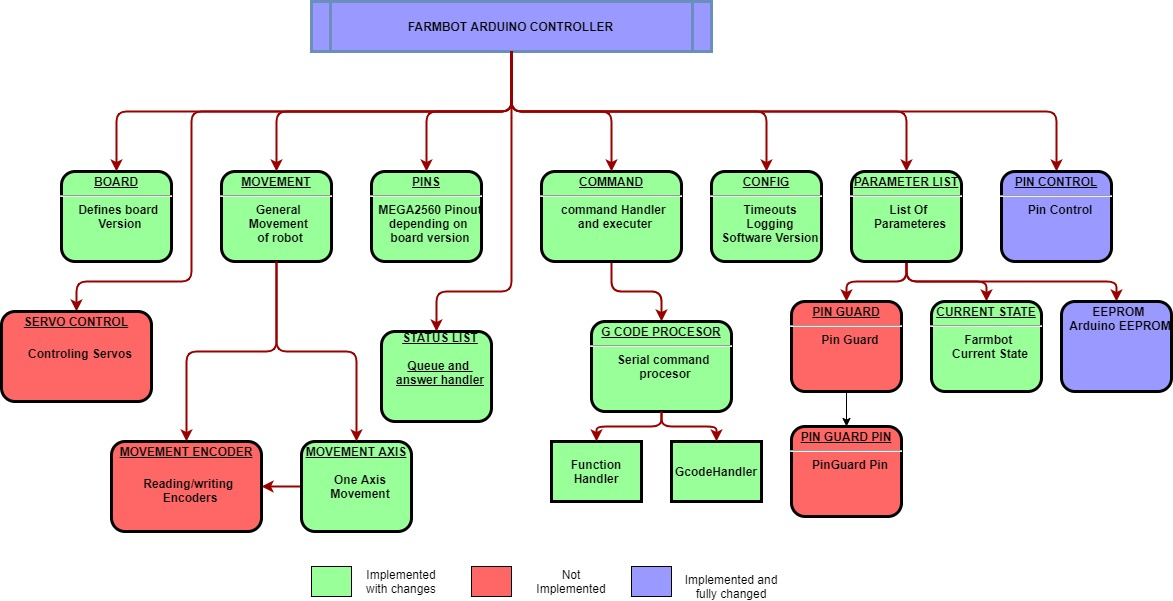
\includegraphics[width=1\linewidth]{images/ArduinoFirmwareFarmbot}
		\label{fig:arduinofirmwarefarmbot}
	\end{figure}
	\subsection{Scheduling}
	En la siguiente figura se muestra el diagrama de hilos para la interfaz, esta solo cuenta con dos hilos, uno que se activa despues de iniciar el farmbo y otro que lo hace cada vez que se ejecuta un comando desde la consola serial.
	\begin{figure}[H]
		\centering
		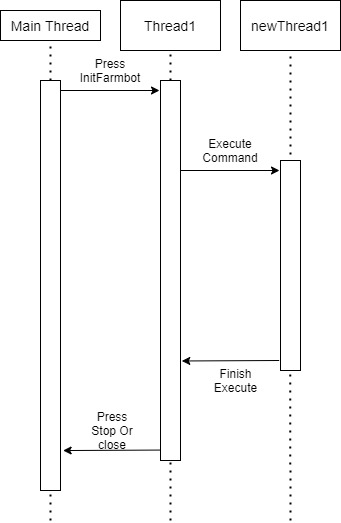
\includegraphics[width=0.5\linewidth]{images/hilos_desarrollador}
		\label{fig:hilosdesarrollador}
	\end{figure}
	
	
	
	\section{Configuración del software requerido}
	\subsection{Instalacion de Visual Studio}
	Este código fue escrito usando visual Studio Professional V19, las instrucciones de descarga e instalación están en el siguiente \href{https://visualstudio.microsoft.com/es/thank-you-downloading-visual-studio/?sku=Professional&rel=16}{link}.
	\subsection{Instalación de Paquetes}
	 Los paquetes que se muestran en la figura deben ser instalados antes de abrir el codigo.
	Para instalar los paquete:
	\begin{itemize}
		\item  Abra VisualStudio Installer
		
		\item En su versión del instalador seleccione More->Modify
		\begin{figure}[H]
			\centering
			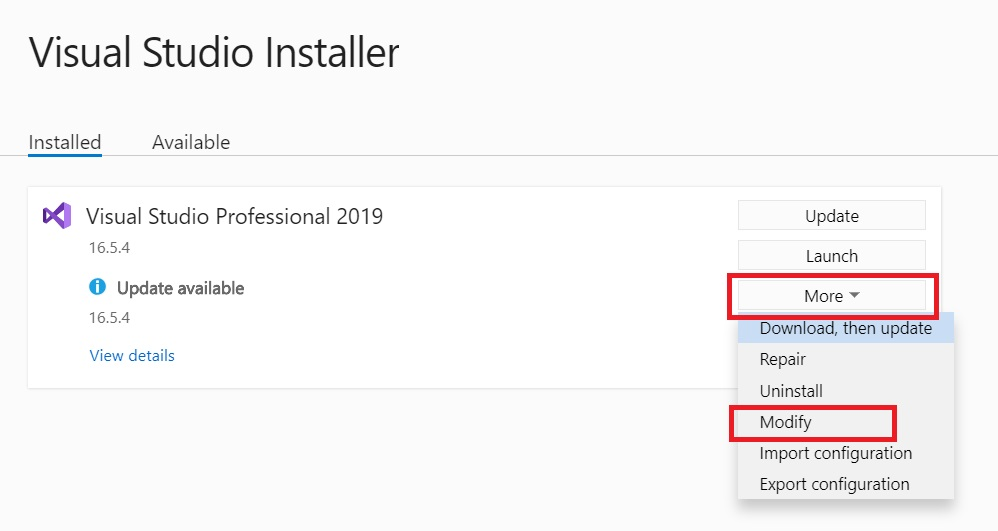
\includegraphics[width=0.7\linewidth]{images/Visual1}
			\label{fig:visual1}
		\end{figure}
		
		\item Seleccione "Individual Components"
		\item Navegue al menú ".NET" y verifique que concuerde con la figura
		\begin{figure}[H]
			\centering
			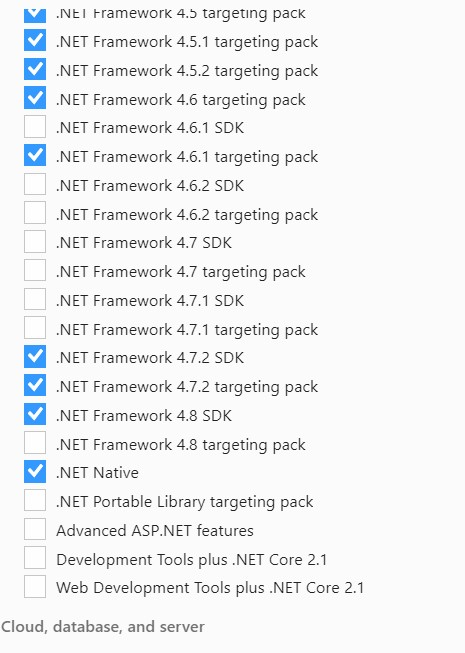
\includegraphics[width=0.7\linewidth]{images/Visual2}
			\label{fig:visual2}
		\end{figure}
		
		\item  Navegue al menú "Compilers, build tools, and runtimes" y verifique que concuerde con las siguientes figuras
		
		\begin{figure}[H]
			\centering
			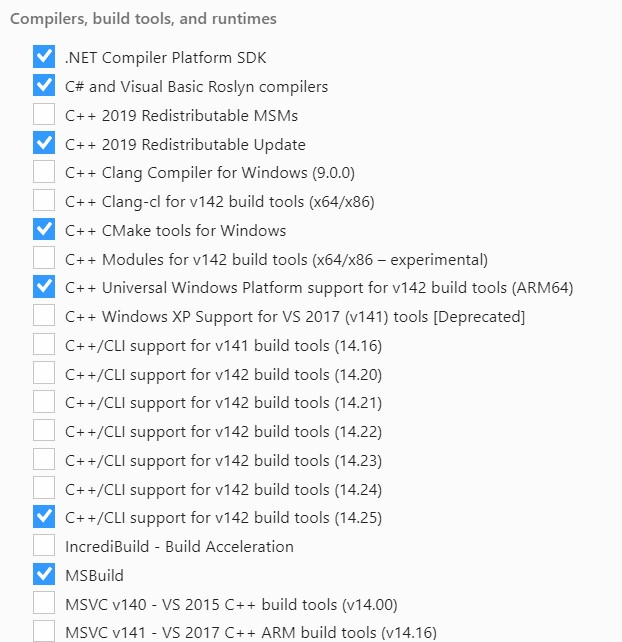
\includegraphics[width=0.7\linewidth]{images/Visual3}
			\label{fig:visual3}
		\end{figure}
	\begin{figure}[H]
		\centering
		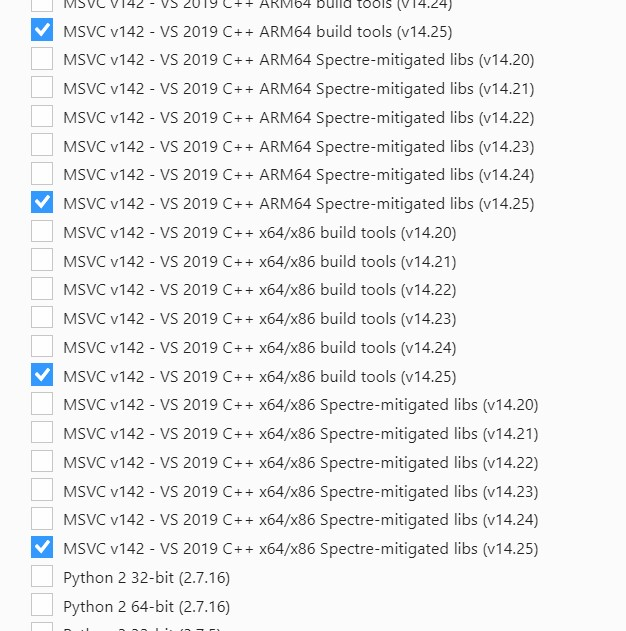
\includegraphics[width=0.7\linewidth]{images/Visual4}
		\label{fig:visual4}
	\end{figure}
	

			
	\end{itemize}  	

\subsection{Configuración del escalamiento}
Una vez abierto el proyecto y teniendo en cuenta que visual Studio es una aplicación que funciona por DPI, al abrir el formulario en forma de diseño este aparecerá escalado mostrando la ventana que se muestra en la figura  
\begin{figure}[H]
	\centering
	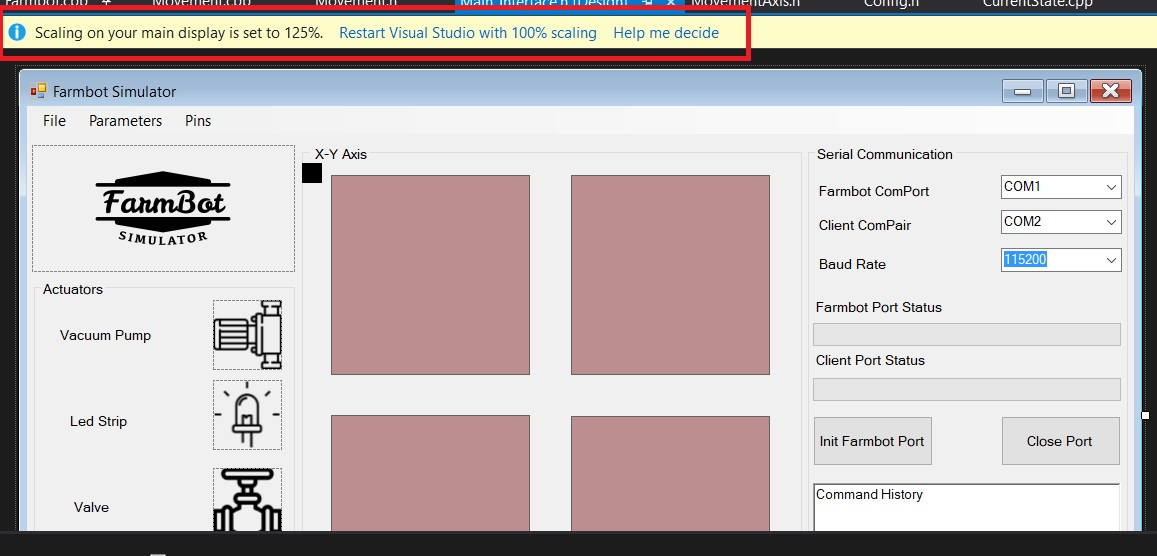
\includegraphics[width=0.7\linewidth]{images/scaling}
	\label{fig:scaling}
\end{figure}
\subsection{Virtual Serial Ports Free}
\label{sec:virtualPort}
El instalador del programa se encuentra en la carpeta llamada "Virtual Serial", para instalarlo ejecute el archivo como administrador del sistema y siga los pasos. Si desea la ultima versión del programa la puede descargar del siguiente \href{https://freevirtualserialports.com/}{link}.El programa corriendo se muestra en la figura.Para configurar los puertos seriales para esta aplicacion realice los siguientes pasos
\begin{itemize}
	\item Abra el programa con permisos de administrador
	\item Haga click en "Continue with limited features"
\begin{figure}[H]
	\centering
	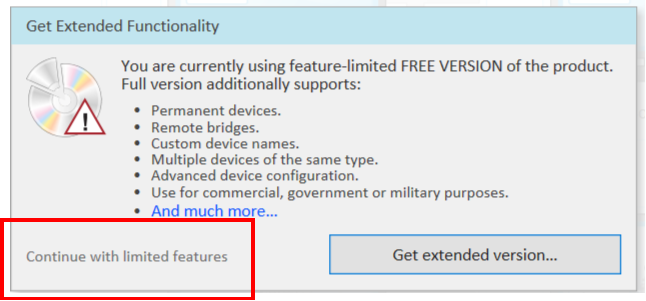
\includegraphics[width=0.7\linewidth]{images/virtual1}

	\label{fig:virtual1}
\end{figure}

	
	\item Haga click en "Create Local Bridge"
	\begin{figure}[H]
		\centering
		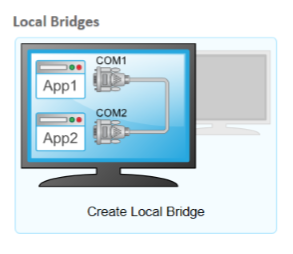
\includegraphics[width=0.5\linewidth]{images/virtual2}
		\label{fig:virtual2}
	\end{figure}
	\item Seleccione los nombres de los puertos, tenga en cuenta estos nombres para posteriormente usarlos en las aplicaciones.
	\begin{figure}[H]
		\centering
		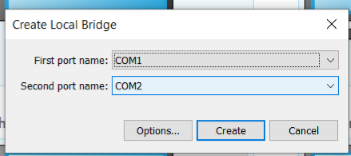
\includegraphics[width=0.5\linewidth]{images/virtual3}
		\caption{}
		\label{fig:virtual3}
	\end{figure}
	\item Presione click en Ok, tenga en cuenta que estos puertos existirán unicamente hasta que reinicie el sistema, es decir cada vez que lo reinicie deberá seguir los pasos anteriormente descritos.
\end{itemize}

	\section{Descripción de los archivos y las clases}
	
	\subsection{ArduinoPins}
	\label{sub_ArduinoPins}

	\subsection{Board}
	Este archivo solo contiene un archivo de cabecera con la declaración de la versión de la board, es decir la pc, para el farmbot existen 4 versiones, su versión mas antigua es la ramps, la segunda y tercera versión es la que se encuentra en el famrbot uniandes actualmente. y la ultima versión que incluye Stepper drivers que se comunican por SPI y que estará en el farmbot para 2020-2. Esta interfaz fue programada usando la versión 1.4 del farmbot.

	
	\subsection{Command}
	Esta clase es la encargada de tomar un String que es el mensaje que se envía por serial y devolver un objeto de tipo comando con el comando que se envió, ademas también tiene métodos que parten ese mismo String para obtener los parámetros que acompañan, como ejemplo si envía el comando "G00 X100 Y100 Z100", al crear un objeto de tipo "Command" con este string, este tendrá las siguientes propiedades:
	\begin{itemize}
		\item CommandCodeEnum G00
		\item long X= 100
		\item Long Y=100
		\item Long Z=100
	\end{itemize}
	Cabe aclarar que esta clase no es la encargada de ejecutar el comando que se envió solo guarda su información.

	\subsection{Config}
	
	Este archivo solo contiene un archivo de cabecera con los parametros del farmbot default asi como las constantes que tienen diferentes mensajes de respuesta del farmbot ( R00,R99, etc). Estos se encuentran definidos para cada una de las versiones.
	
	\subsection{CurrentState}
	Esta clase contiene el estado actual del farmbot es decir:
	\begin{itemize}
		\item La posición actual en los 3 ejes
		\item La posición de la cola de ejecución de comandos
		\item El estado de emergencia (si se encuentra en emergencia o no)
		\item La conversión de pasos a mm 
	\end{itemize}
	Ademas esta clase permite acceder a los valores anteriormente mencionados mediante métodos get y cambiarlos mediante métodos set.Como funcionalidad adicional tiene el método "PrintQAndNewline" que imprime por serial los caracteres que se ponen al final de cada mensaje.
	\subsection{F09-F84 Handler}
	\label{sub_F}
	Estos son varios archivos, cada uno ejecuta la función que lleva por nombre con los parámetros que necesita para ejecutarla a los cuales accede a través del comando que recibe como parámetro en su instancia-miento y los métodos get de la clase current state. Cada una de estas funciones es de tipo "GCodeHnadler"
	\subsection{G00 and G28 Handler}
	\label{sub_G}
		Estos son varios archivos, cada uno ejecuta la función de movimiento que lleva por nombre con los parámetros que necesita para ejecutarla a los cuales accede a través del comando que recibe como parámetro en su instancia-miento y los métodos get de la clase current state. Cada una de estas funciones es de tipo "GCodeHnadler"
	\subsection{GCodeHandler}
	Esta clase esta escrita como un "plantilla" para las clases F y las clases G, unicamente cuenta con el comando "execute" y establece el modelo para las demas, ya que las clases descritas en la sección \ref{sub_} y \ref{sub_F} son de este tipo deben seguir su mismo modelo
	
	\subsection{GCodeProcessor}
	Esta clase es la encargada de recibir el comando por string, convertir ese string en un comando, tomar el comando y según su "CommandCodeEnum" crear un objeto de tipo GCodeHandler que tiene la función especifica y correr el método execute de esta función.
	\subsection{MainInterface}
	Clase con la interfaz de usuario, esta clase puede decirse que es la principal, ya que esta crea una instancia del farmbot, ademas que es a la que se entra desde el main. Una particularidad de esta clase es que esta escrita en C++/CLI usando .NET 4.7.2 por lo que se debe tener en cuenta el tipo de clase que es y particularidades, en el siguiente \href{https://geeks.ms/rfog/2009/06/15/qu-es-c-y-qu-es-ccli/}{link} encontrara las diferencias entre C++ y C++/CLI, como se conecta con .NET y como manejar ambos lenguajes.
	\subsection{MovementAxis}
	Clase encargada del movimiento de un eje, cuenta con los métodos para saber si el eje esta en home o si ya llego a su destino. Ademas en este se incluyo la simulación de la velocidad del farmbot usando el tiempo del sistema y las constantes de velocidad par saber cuantos pasos debía moverse en una ventana pequeña de tiempo de 10 ms
	\subsection{Movement}
	Movimiento general del robot, incluye 3 variables de tipo MovemementAxis, una para cada eje. esta se encarga de que el Farmbot llegue a su destino en los 3 puntos usando los métodos de validación de MovementAxis
	\subsection{ParameterList}
	Clase con la lectura y escritura de parámetros del Farmbot. Los parametros son originalmente guardados en la EEPROM de arduino, al no tener ese recurso disponible se guardó en el disco duro del sistema usando archivos CSV.
	\subsection{PinClass}
	Clase que sustituye los pines físicos del arduino, esta clase crea objetos de tipo pin que tienen un valor y se define si son de entrada o salida etc como si estos fueran los pines físicos del arduino, pudiendo acceder a sus valores desde la clase ArduinoPins explicada en \ref{sub_ArduinoPins}
	\subsection{PinControl}
	Clase encargada del control de pines físicos del arduino, no utilizada en este codigo, pero se mantuvo para evitar errores en declaraciones ya que el archivo cuenta con algunas constantes
	\subsection{Pins}
		Este archivo solo contiene un archivo de cabecera con la declaración de los pines del arduino en función de la versión de la board, es decir, el nombre y el numero de pin donde irían conectados los actuadores y sensores del farmbot.
	\subsection{StatusList}
	Esta clase se encargaba de escribir y leer los pines del arduino así como del pinguard usando la clase pincontrol, como pincontrol no fue implementada, esta clase tampoco. La sustitución de esta clases en modo simulación fue implementada en la \ref{sub_ArduinoPins}
	\section{Probando el código}
	En el siguiente \href{URL}{video} puede encontrar una prueba de funcionamiento del Farmbot usando la interfaz de python, en caso de que no quiera usar la interfaz puede usar cualquier monitor serial como el de arduino y enviar los comandos manualmente teniendo en cuenta los puertos virtuales que creo en la sección \ref{sec:virtualPort}, la descripción de los comandos la encuentra en la pagina del Farmbot en el siguiente \href{URL}{link}
	\section{Trabajos futuros}
	Algunos trabajos futuros que podrían ser implementados para mejorar el performance de esta interfaz son: 
	\begin{itemize}
		\item \textbf{Incluir mutex:} esta clase es usada en el threading para evitar que dos hilos accedan a la misma variable al mismo tiempo.Para este caso las variables a las que podría acceder el programa al mismo tiempo desde diferentes hilos  son las posiciones. Sin embargo debido al desarrollo y timing de los hilos es poco probable que estos accedan a la misma variable pero es un aspecto a tener en cuenta.
		\item \textbf{Validación de final de eje:}El farmbot original gracias a los encoder puede parar cuando llego al final del eje, al no tener estos en el farmbot simulator debe implementarse alguna estrategia para verificar que se llego al final,esta podría ser calcular el largo del eje en pasos y comparar con el numero de pasos dados por cada eje.
	\end{itemize}


\end{document}